\chapter{Математическая модель БОЭП и его составных частей как объекта управления} \label{ch:ch3}

Оптико-электронный прибор (ОЭП) вертолетного базирования имеет тепловизионный и телевизионный каналы, лазерный дальномер. Кроме того, на борту устанавливают оптико-электронную систему постановки помех (СОЭП).  Управление направлением линии визирования осуществляется перемещением всего оптико-электронного блока. Для ОЭП и СОЭП конструктивно оптико-электронный блок представляет собой блок, в котором размещены оптические приборы, вращающийся по углу места внутри вилки, вращающейся по углу азимута 
(рисунок~\ref{fig:device}, кинематическая схема на рисунке~\ref{fig:kinematic}). 
На осях вращения размещены моментные двигатели и датчики углов. ОЭП установлен в носовой части вертолета, СОЭП устанавливается в хвостовой части и на балках 
(рисунок~\ref{fig:helicopter}).

При проектировании ОЭП и СОЭП возникли задачи построения адекватной математической модели, синтеза системы управления направлением линии визирования и построения компьютерной имитационной модели ОЭП и СОЭП. Решение этих задач является продолжением работ [3/15-18]. Математическая модель строится на основе применения уравнений Лагранжа II-го рода с использованием смешанного метода Жильбера. Разработаны алгоритмы управления, обеспечивающие требуемые точностные и динамические характеристики СОЭП для режима слежения и наведения. Исследование динамических свойств СОЭП проводится с использованием компьютерной имитационной модели. Использование метода математического моделирования при проектировании бортовых СОЭП позволяет обеспечить достижение заложенных технических требований по параметрам системы, сократить сроки разработки, настройки и испытаний изделия. Компьютерная имитационная модель верифицирована по результатам настройки опытного образца.

\begin{landscape}
\section{Принципиальная схема} \label{ch:ch3/sect1}

\begin{figure}[ht]
	\centering
	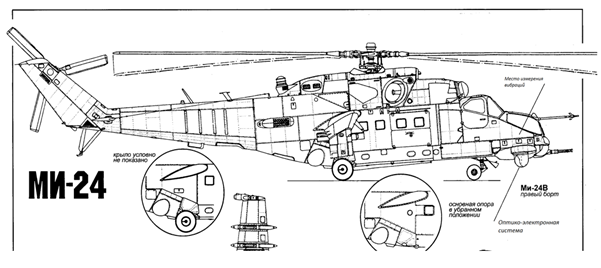
\includegraphics[width=0.9\linewidth]{img-15} 
	\caption{Принципиальная схема расположения на борту}
	\label{fig:helicopter}
\end{figure}

\begin{figure}[ht]
	\centering
	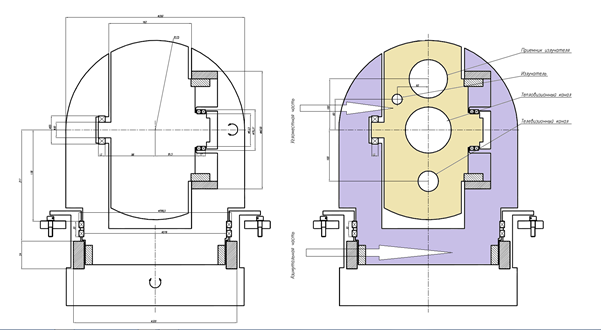
\includegraphics[width=0.9\linewidth]{img-16} 
	\caption{Общий вид изделия}
	\label{fig:device}
\end{figure}
\end{landscape}

\section{Механическая модель} \label{ch:ch3/sect2}

Исходя из анализа конструкции ОЭП для управления линией визирования оптико-электронного блока – объекта управления (ОУ) и движения вертолета (ЛА), на котором он установлен, приняты основные допущения, выбраны системы координат и определены исходные данные, необходимые для построения математической модели. ОУ.

\begin{figure}[ht]
	\centering
	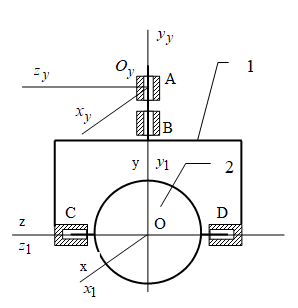
\includegraphics[]{img-17} 
	\caption{Кинематическая схема}
	\label{fig:kinematic}
\end{figure}

\subsection{Основные допущения, системы координат} \label{sec:ch3/sec3}

\begin{enumerate}
	\item ОУ моделируется двумя абсолютно твердыми телами:
	\begin{itemize}
		\item 1–е тело объединяет все элементы, вращающиеся по углу азимута вокруг оси АВ (рисунок \ref{fig:kinematic}) в неограниченном диапазоне (более $360_0$). Тело 1 (вилка) совершает вращательное движение вокруг оси АВ под действием вращающего момента, создаваемого моментным двигателем.
		\item 2–е тело (оптико-электронный блок) объединяет все элементы, вращающиеся по углу места вокруг оси CD (рисунок \ref{fig:device}). Тело 2 (оптико-электронный блок) вращается относительно тела 1 вокруг оси CD под действием вращающего момента, создаваемого другим моментным двигателем.
	\end{itemize}
	\item Ось вращения 2-го тела перпендикулярна оси вращения 1-го тела и пересекается с ней: $AB\perp CD$, т.$O \in AB$, т.$O \in CD$
	\item Инерциальная система координат, система координат связанная с вертолетом (ЛА) и установочная система координат выбраны в соответствии с принципиальной схемой расположения на борту (рисунок \ref{fig:helicopter}). Их положение и кинематические характеристики  определены выражениями (3.1)-(3.14).
	\item Система координат $O_{x_1y_1z_1}$ (рисунок \ref{fig:coord/3.4}) жестко связана с 1-м телом. 
	\begin{figure}[ht]
		\centering
		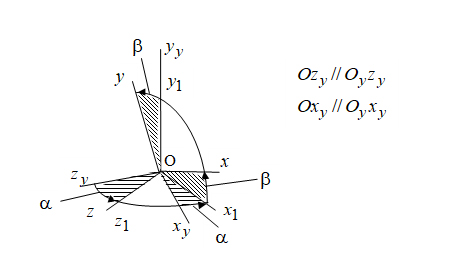
\includegraphics[]{img-18} 
		\caption{Кинематическая схема}
		\label{fig:coord/3.4}
	\end{figure}

	Ось $O_{y_1}$ направлена по оси вращения АВ, ось $O_{z_1}$ направлена по оси вращения CD, ось $O_{x_1}$ дополняет указанные оси до правой системы координат. Точка O находится на пересечении осей АВ и CD. Положение точки О в установочной системе координат определяется радиусом-вектором
	\begin{equation}
	\label{eq:p3:1}
	\begin{alignedat}{2}
	\bar{r}_0 = \bar{e}_y\tilde{r}_0 ,
	\end{alignedat}
	\end{equation}
	где $\tilde{r}_0 = (0 -l 0)^T$.
	
	Орты осей $O_{x_1y_1z_1}$ обозначим $\bar{i}_1$, $\bar{j}_1$, $\bar{k}_1$ и составим из них базисную строку $\bar{e}_1 = (\bar{i}_1 \bar{j}_1 \bar{k}_1)$. Связь между базисными строками $\bar{e}_y$ и $\bar{e}_1$ определяются матрицей $A_1$:
	\begin{equation}
	\label{eq:p3:2}
	\begin{alignedat}{2}
	\bar{e}_y = \bar{e}_1	A_1 ,
	\end{alignedat}
	\end{equation}
	где  \( A_{1}= \left( \begin{matrix}
	cos \alpha   &  0  &  -sin \alpha \\
	0  &  1  &  0\\
	sin \alpha   &  0  &  cos \alpha \\
	\end{matrix}
	\right)  \) .\par
	
	Масса 1-го тела равна  \( m_{1} \) , положение центра масс в системе координат  \( Ox_{1}y_{1}z_{1} \)  определяется радиусом-вектором\par
	
	\begin{equation}
	\label{eq:p3:3}
	\begin{alignedat}{2}
	r_{с_{1}}=e_{1}r_{с_{1}},
	\end{alignedat}
	\end{equation}
	
	где  \( r_{с_{1}}= \left( \begin{matrix}
	x_{с_{1}}  &  y_{с_{1}}  &  z_{с_{1}}\\
	\end{matrix}
	\right) ^{T} \) .\par
	Введем следующие обозначения для осевых и центробежных моментов инерции 1-го тела:\par
	
	\( J_{x_{1}}=A_{1},J_{y_{1}}=B_{1},J_{z_{1}}=C_{1},J_{x_{1}y_{1}}=F_{1},J_{x_{1}z_{1}}=E_{1},J_{y_{1}z_{1}}=D_{1} \) ,\par
	
	тогда его тензор инерции\par
	
	\begin{equation}
	\label{eq:p3:4}
	\begin{alignedat}{2}
	J_{1}= \left( \begin{matrix}
	A_{1}  &  -F_{1}  &  -E_{1}\\
	-F_{1}  &  B_{1}  &  -D_{1}\\
	-E_{1}  &  -D_{1}  &  C_{1}\\
	\end{matrix}
	\right) 
	\end{alignedat}
	\end{equation}
		
	\item Оси  \( Oxyz \)  (рисунок \ref{fig:coord/3.4}) жестко связаны с телом 2: ось  \( Ox \)  направлена по оптической оси, ось  \( Oz \)  совпадает с осью вращения \textit{CD}, ось  \( Oy \)  дополняет указанные оси до правой системы координат.\par
	
	Орты осей  \( Ox_{1}y_{1}z_{1} \)  обозначим  \( i,j,k_{1} \)  и составим из них базисную строку  \( е= \left( \begin{matrix}
	i  &  j  &  k\\
	\end{matrix}
	\right)  \) . Связь между базисными строками  \( e \)  и  \( e_{1} \)  определяется матрицей  \( A_{2} \) :\par
	
	\begin{equation}
	\label{eq:p3:5}
	\begin{alignedat}{2}
	e_{1}=eA_{2},
	\end{alignedat}
	\end{equation}
	
	где  \( A_{2}= \left( \begin{matrix}
	cos \beta   &  sin \beta   &  0\\
	-sin \beta   &  cos \beta   &  0\\
	0  &  0  &  1\\
	\end{matrix}
	\right)  \) .\par
	
	Масса 2-го тела равна  \( m_{2} \) , положение центра масс в системе координат  \( Oxyz \)  определяется радиусом-вектором\par
	
	\begin{equation}
	\label{eq:p3:6}
	\begin{alignedat}{2}
	r_{с_{2}}=e r_{с_{2}},
	\end{alignedat}
	\end{equation}
	
	где  \( r_{с_{2}}= \left( \begin{matrix}
	x_{с_{2}}  &  y_{с_{2}}  &  z_{с_{2}}\\
	\end{matrix}
	\right) ^{T} \) .\par
	
	Введем следующие обозначения для осевых и центробежных моментов инерции 2-го тела:\par
	
	\( J_{x_{}}=A_{2},J_{y}=B_{2},J_{z}=C_{2},J_{x_{2}y_{2}}=F_{2},J_{x_{2}z_{2}}=E_{2},J_{y_{2}z_{2}}=D_{2} \) ,\par
	
	тогда его тензор инерции\par
	
	\begin{equation}
	\label{eq:p3:7}
	\begin{alignedat}{2}
	J_{2}= \left( \begin{matrix}
	A_{2}  &  -F_{2}  &  -E_{2}\\
	-F_{2}  &  B_{2}  &  -D_{2}\\
	-E_{2}  &  -D_{2}  &  C_{2}\\
	\end{matrix}
	\right) 
	\end{alignedat}
	\end{equation}	
	\item Движение ЛА происходит в однородном поле силы тяжести.
\end{enumerate}


\subsection{Геометрия масс} \label{sec:ch3/sec4}

По рабочим чертежам в среде Solid Works получены массовые характеристики ОУ. Их обозначения и величины приведены в таблице ниже (таблица \ref{tab:MASS/3.1}).



{
	\setlength\extrarowheight{3pt}
	\begin{longtable}{p{0.66in}p{1.94in}p{0.71in}p{0.29in}p{0.49in}p{0.39in}p{0.66in}}
		\caption{Массовые характеристики ОУ}%
		\label{tab:MASS/3.1}% label всегда желательно идти после caption
		\\
\hline
		%row no:1
		\multicolumn{1}{|p{0.66in}}{№ п/п} & 
		\multicolumn{1}{|p{1.94in}}{Наименование} & 
		\multicolumn{1}{|p{0.71in}}{Обозначение} & 
		\multicolumn{3}{|p{1.57in}}{Величина} & 
		\multicolumn{1}{|p{0.66in}|}{Размерность} \\
		\hline
		%row no:2
		\multicolumn{1}{|p{0.66in}}{1} & 
		\multicolumn{1}{|p{1.94in}}{2} & 
		\multicolumn{1}{|p{0.71in}}{3} & 
		\multicolumn{3}{|p{1.57in}}{4} & 
		\multicolumn{1}{|p{0.66in}|}{5} \\
		\hline
		%row no:3
		\multicolumn{1}{|p{0.66in}}{1} & 
		\multicolumn{1}{|p{1.94in}}{Координаты центра прибора относительно центра масс носителя \par } & 
		\multicolumn{1}{|p{0.71in}}{Y\textsubscript{0} \par X\textsubscript{0} \par Z\textsubscript{0}} & 
		\multicolumn{1}{|p{0.29in}}{-0.5 \par -0.5 \par -2} & 
		\multicolumn{1}{|p{0.49in}}{0 \par -8.422 \par 0} & 
		\multicolumn{1}{|p{0.39in}}{-0.5 \par -0.5 \par 2} & 
		\multicolumn{1}{|p{0.66in}|}{\textit{м}} \\
		\hline
		%row no:4
		\multicolumn{1}{|p{0.66in}}{2} & 
		\multicolumn{1}{|p{1.94in}}{\multirowcell{2}{}{\begin{tabular}{p{1.94in}}Масса 1-го тела вращения (по азимуту), координаты его центра масс, осевые и центробежные моменты инерции\\(Ось вращения – Y)\\\end{tabular}}} & 
		\multicolumn{1}{|p{0.71in}}{m\textsubscript{1}} & 
		\multicolumn{3}{|p{1.57in}}{15.7} & 
		\multicolumn{1}{|p{0.66in}|}{\textit{кг}} \\
		\hline
		%row no:5
		\multicolumn{1}{|p{0.66in}}{3} & 
		\multicolumn{1}{|p{1.94in}}{} & 
		\multicolumn{1}{|p{0.71in}}{x\textsubscript{C1}} & 
		\multicolumn{3}{|p{1.57in}}{-2.82} & 
		\multicolumn{1}{|p{0.66in}|}{\textit{мм}} \\
		\hline
		%row no:6
		\multicolumn{1}{|p{0.66in}}{4} & 
		\multicolumn{1}{|p{1.94in}}{} & 
		\multicolumn{1}{|p{0.71in}}{z\textsubscript{C1}} & 
		\multicolumn{3}{|p{1.57in}}{8.64} & 
		\multicolumn{1}{|p{0.66in}|}{\textit{мм}} \\
		\hline
		%row no:7
		\multicolumn{1}{|p{0.66in}}{5} & 
		\multicolumn{1}{|p{1.94in}}{} & 
		\multicolumn{1}{|p{0.71in}}{y\textsubscript{C1}} & 
		\multicolumn{3}{|p{1.57in}}{-95.03} & 
		\multicolumn{1}{|p{0.66in}|}{\textit{мм}} \\
		\hline
		%row no:8
		\multicolumn{1}{|p{0.66in}}{6} & 
		\multicolumn{1}{|p{1.94in}}{} & 
		\multicolumn{1}{|p{0.71in}}{ \( J_{x_{1}}=A_{1} \) } & 
		\multicolumn{3}{|p{1.57in}}{212} & 
		\multicolumn{1}{|p{0.66in}|}{\textit{гр м\textsuperscript{2}}} \\
		\hline
		%row no:9
		\multicolumn{1}{|p{0.66in}}{7} & 
		\multicolumn{1}{|p{1.94in}}{} & 
		\multicolumn{1}{|p{0.71in}}{ \( J_{y_{1}}=B_{1} \) } & 
		\multicolumn{3}{|p{1.57in}}{311.8} & 
		\multicolumn{1}{|p{0.66in}|}{\textit{гр м\textsuperscript{2}}} \\
		\hline
		%row no:10
		\multicolumn{1}{|p{0.66in}}{12} & 
		\multicolumn{1}{|p{1.94in}}{\multirowcell{2}{}{\begin{tabular}{p{1.94in}}Масса 2-го тела вращения (по углу места), координаты его центра масс, осевые и центробежные моменты инерции\\(Ось вращения - Z)\\\end{tabular}}} & 
		\multicolumn{1}{|p{0.71in}}{ \( m_{2} \) } & 
		\multicolumn{3}{|p{1.57in}}{1130.85} & 
		\multicolumn{1}{|p{0.66in}|}{\textit{гр}} \\
		\hline
		%row no:11
		\multicolumn{1}{|p{0.66in}}{13} & 
		\multicolumn{1}{|p{1.94in}}{} & 
		\multicolumn{1}{|p{0.71in}}{ \( x_{C_{2}} \) } & 
		\multicolumn{3}{|p{1.57in}}{0} & 
		\multicolumn{1}{|p{0.66in}|}{\textit{мм}} \\
		\hline
		%row no:12
		\multicolumn{1}{|p{0.66in}}{14} & 
		\multicolumn{1}{|p{1.94in}}{} & 
		\multicolumn{1}{|p{0.71in}}{ \( y_{C_{2}} \) } & 
		\multicolumn{3}{|p{1.57in}}{14.8} & 
		\multicolumn{1}{|p{0.66in}|}{\textit{мм}} \\
		\hline
		%row no:13
		\multicolumn{1}{|p{0.66in}}{15} & 
		\multicolumn{1}{|p{1.94in}}{} & 
		\multicolumn{1}{|p{0.71in}}{ \( z_{C_{2}} \) } & 
		\multicolumn{3}{|p{1.57in}}{-8} & 
		\multicolumn{1}{|p{0.66in}|}{\textit{мм}} \\
		\hline
		%row no:14
		\multicolumn{1}{|p{0.66in}}{16} & 
		\multicolumn{1}{|p{1.94in}}{} & 
		\multicolumn{1}{|p{0.71in}}{ \( J_{x_{2}}=A_{2} \) } & 
		\multicolumn{3}{|p{1.57in}}{3.3} & 
		\multicolumn{1}{|p{0.66in}|}{\textit{гр м\textsuperscript{2}}} \\
		\hline
		%row no:15
		\multicolumn{1}{|p{0.66in}}{17} & 
		\multicolumn{1}{|p{1.94in}}{} & 
		\multicolumn{1}{|p{0.71in}}{ \( J_{y_{2}}=B_{2} \) } & 
		\multicolumn{3}{|p{1.57in}}{7.5} & 
		\multicolumn{1}{|p{0.66in}|}{\textit{гр м\textsuperscript{2}}} \\
		\hline
		%row no:16
		\multicolumn{1}{|p{0.66in}}{18} & 
		\multicolumn{1}{|p{1.94in}}{} & 
		\multicolumn{1}{|p{0.71in}}{ \( J_{z_{2}}=C_{2} \) } & 
		\multicolumn{3}{|p{1.57in}}{8.4} & 
		\multicolumn{1}{|p{0.66in}|}{\textit{гр м\textsuperscript{2}}} \\
		\hline
		
\end{longtable}}

%%%%%%%%%%%%%%%%%%%% Table No: 4 ends here %%%%%%%%%%%%%%%%%%%%

\section{Составление уравнений динамической модели ОУ} \label{ch:ch3/sect5}

ОУ моделируется двумя абсолютно твердыми телами (тело 1 и тело 2), установленными в корпусе, который закреплен на ЛА. Положение этих тел относительно корпуса однозначно определяется углами поворотов:  \(  \alpha  \)  и  \(  \beta  \) . К активным силам, действующим на ОЭП, отнесем силы тяжести, момент от азимутального привода – моментного двигателя, момент от угломестного привода – второго моментного двигателя, моменты трения. Тогда связи, ограничивающие перемещения указанных тел, можно считать идеальными. Кроме того, связи являются голономными, удерживающими и стационарными. Для построения математической модели относительного движения ОУ в установочной системе координат (движения относительно корпуса) будем использовать уравнения Лагранжа II-го рода. Метод их составления для относительного движения объекта, установленного на подвижном основании, описан в разделе \ref{ch:ch3/sect1}. Механическая модель. Он состоит из трех этапов: вычисления кинетической энергии, вычисления обобщенных сил и составления уравнений движения (проведения действий в соответствии с уравнениями Лагранжа II-го рода). За обобщенные координаты принимаются углы поворота:  \( q_{1}= \alpha ,q_{2}= \beta  \) .\par





\subsection{Вычисление кинетической энергии} \label{sec:ch3/sec6}

В соответствии с выражением (3.23) вычислим кинетическую энергию ОУ, находящемся на ЛА, совершающем произвольный маневр, в соответствии с уравнениями (\labelcref{eq:p3:1}). Вектор ускорения центра масс ЛА, вектор угловой скорости и вектор углового ускорения определяются соответственно выражениями (\labelcref{eq:p3:5,eq:p3:7}). Будем учитывать вибрацию установочной системы координат, которая задается уравнениями (\labelcref{eq:p3:9}).

Кинетическая энергия ОЭС в относительном движении в установочных осях  \( Ox_{y}y_{y}z_{y} \)  (тело 1 совершает вращательное движение, тело 2 – сферическое) определяется следующим образом:\par

\begin{equation}
\label{eq:p3:8}
\begin{alignedat}{2}
T_{r}= \sum_{j=1}^{2}T_{r}^{ \left( j \right) }= \sum_{j=1}^{2}\frac{1}{2} \left(  \omega_{j}^{r} \right) ^{T}J_{j} \omega_{j}^{r}
\end{alignedat}
\end{equation}

здесь  
\( J_{j} \) – тензор инерции и  
\(  \omega_{j}^{r} \) – координатный вектор относительной угловой скорости \textit{j}–го тела в системе координат, связанной с этим телом.\par


Векторы угловых скоростей 1-го и 2-го тел в установочной системе координат  \( Ox_{y}y_{y}z_{y} \)  определяются в соответствии с изображением систем координат (рисунок~\ref{fig:coord/3.4}). Угловая скорость 1-го тела \par

\begin{equation}
\label{eq:p3:9}
\begin{alignedat}{2}
\omega_{1}^{r}=e_{1} \omega_{1}^{r}=e_{1} \left( \begin{matrix}
0\\
\alpha \\
0\\
\end{matrix}
\right) ,
\end{alignedat}
\end{equation}

угловая скорость 2-го тела\par

\begin{equation}
\label{eq:p3:10}
\begin{alignedat}{2}
 \omega_{2}^{r}=e_{2} \omega_{2}^{r}=e_{2} \left( \begin{matrix}
\alpha sin \beta \\
\alpha cos \beta \\
\beta \\
\end{matrix}
\right) .
\end{alignedat}
\end{equation}

С учетом принятых обозначений (\labelcref{eq:p3:4}) и (\labelcref{eq:p3:7}), а также выражений (\labelcref{eq:p3:9}),(\labelcref{eq:p3:10}), после проведения действий в соответствии с (\labelcref{eq:p3:8}) находим\par

\begin{equation}
\label{eq:p3:11}
\begin{alignedat}{2}
T_{r}=
\frac{1}{2} 
[  
	( 
		B_{1}+
		A_{2}sin^{2} (  \beta  ) +
		B_{2}cos^{2} (  \beta  ) -
		F_{2}sin ( 2 \beta  )  
	)  \dot{\alpha}^{2} + \\
	C_{2} \dot{\beta}^{2} -  
	2 ( 
		E_{2}sin (  \beta  ) +
		D_{2}cos (  \beta  )  
	)  
	\dot{\alpha}  \dot{\beta}  
] 
\end{alignedat}
\end{equation}

Кинетический момент ОУ относительно точки \textit{О} в относительном движении в установочных осях  \( Ox_{y}y_{y}z_{y} \)  равен\par

\begin{equation}
\label{eq:p3:12}
\begin{alignedat}{2}
\bar{K}_{O}^{r}= \sum_{j=1}^{2}\bar{e}_{j}J_{j} \tilde{\omega}_{j}^{r}
\end{alignedat}
\end{equation}

Из выражений (\labelcref{eq:p3:2}), (\labelcref{eq:p3:5}), учитывая то, что матрицы в этих выражениях являются ортогональными, имеем\par

\begin{equation}
\label{eq:p3:13}
\begin{alignedat}{2}
\bar{e}_{1} = \bar{e}_{y} A_{1}^{T} ,
\bar{e}_{2} = 
\bar{e} = 
\bar{e}_{1}A_{2}^{T} = 
e_{y}A_{1}^{T}A_{2}^{T} ,
\end{alignedat}
\end{equation}

Тогда\par

\begin{equation}
\label{eq:p3:14}
\begin{alignedat}{2}
\dot{K}_{O}^{r}=e_{y} [ 
	A_{1}^{T}J_{1} \tilde{\omega}_{1}^{r} + A_{1}^{T} A_{2}^{T} J_{2} \tilde{\omega}_{2}^{r} 
] 
\end{alignedat}
\end{equation}

С учетом принятых обозначений (\labelcref{eq:p3:4}),(\labelcref{eq:p3:7}) и выражений (\labelcref{eq:p3:9}),(\labelcref{eq:p3:10}), после проведения действий в соответствии с (\labelcref{eq:p3:14}) получим\par

\begin{equation}
\label{eq:p3:15}
\begin{alignedat}{2}
\bar{K}_{O}^{r}=\bar{e}_{y}\tilde{K}_{O}^{r}=\bar{e}_{y} \left( \begin{matrix}
K_{x_{y}}^{r} \left( q,q \right) \\
K_{y_{y}}^{r} \left( q,q \right) \\
K_{z_{y}}^{r} \left( q,q \right) \\
\end{matrix}
\right) 
\end{alignedat}
\end{equation}

где \par

\( q= \left( \begin{matrix}
\alpha \\
\beta \\
\end{matrix}
\right)  \) ,\ \ \   \( \dot{q}= \left( \begin{matrix}
\dot{\alpha} \\
\dot{\beta} \\
\end{matrix}
\right)  \) \par

\[
K_{x_{y}}^{r} ( q,\dot{q} ) = 
[
	-( 
		F_{1}cos (  \alpha  ) +
		D_{1}sin (  \alpha  )  
	) +  \]\\ \[
	( 
		\frac{A_{2}-B_{2}}{2}sin ( 2 \beta  ) -
		F_{2}cos ( 2 \beta  )  
	) cos (  \alpha  ) \]\\ \[
	- ( 
		E_{2}sin (  \beta  ) +
		D_{2}cos (  \beta  )  
	) sin (  \alpha  )  
] \dot{\alpha} + \]\\ \[
[
	- ( 
		E_{2}cos (  \beta  ) -
		D_{2}sin (  \beta  )  
	) cos (  \alpha  ) +
	C_{2}sin (  \alpha  )  
]  \dot{\beta}	
\]

\[ K_{y_{y}}^{r} \left( q,q \right) = \left\{ B_{1}+A_{2}sin^{2} \left(  \beta  \right) +B_{2}cos^{2} \left(  \beta  \right) -F_{2}sin \left( 2 \beta  \right)  \right}  \alpha - \] \\ \[ - \left( E_{2}sin \left(  \beta  \right) +D_{2}cos \left(  \beta  \right)  \right)  \beta ; \] \par

\[ K_{z_{y}}^{r} \left( q,q \right) = \left\{  \left( F_{1}sin \left(  \alpha  \right) \frac{}{}D_{1}cos \left(  \alpha  \right)  \right) -  \] \\ \[ - \left( \frac{A_{2}-B_{2}}{2}sin \left( 2 \beta  \right) -F_{2}cos \left( 2 \beta  \right)  \right) sin \left(  \alpha  \right)  \left( \frac{}{} \left( E_{2}sin \left(  \beta  \right) +D_{2}cos \left(  \beta  \right)  \right) cos \left(  \alpha  \right)  \right}  \alpha + \] \\ \[ + \left\{ \frac{}{} \left( E_{2}cos \left(  \beta  \right) -D_{2}sin \left(  \beta  \right)  \right) sin \left(  \alpha  \right) +C_{2}cos \left(  \alpha  \right)  \right}  \beta . \] \par


Вектор угловой скорости установочной системы координат  \( Ox_{y}y_{y}z_{y} \)  в системе координат  \( OXYZ \) \ (переносного движения) определяется суммой угловых скоростей ЛА  и вибрацией установочной системы координат:\par






\begin{equation} %\tag{3.16}
\label{eq:p3:16}
\omega = \omega_{ЛА}+ \omega_{вибр}=e_{c} \omega_{c}+e_{y} \omega_{вибр}=e_{y} \left( A_{y} \omega_{c}+ \omega_{вибр} \right) =e_{y} \omega ==e_{y} \left( \begin{matrix}
\omega_{x_{y}}  &   \omega_{y_{y}}  &   \omega_{z_{y}}\\
\end{matrix}
\right) ^{T}.
\end{equation}
С учетом (\labelcref{eq:p3:15}) и (\labelcref{eq:p3:16}) определим кинетическую энергию\par


\begin{equation} %\tag{3.17}
\label{eq:p3:17}
T_{e}= 
\sum_{j=1}^{2} \omega \left( K_{O}^{r} \right)^{ \left( j \right) }= 
\omega K_{O}^{r}= 
\omega^{T}K_{O}^{r}= 
\omega_{x_{y}}K_{x_{y}}^{r}+ \omega_{y_{y}}K_{y_{y}}^{r}+ \omega_{z_{y}}K_{z_{y}}^{r}
\end{equation}
Вычислим составляющую кинетической энергии \par


\begin{equation} %\tag{3.18}
\label{eq:p3:18}
T^{\ast}= \sum_{j=1}^{2}\frac{1}{2} \omega_{j}^{T}J^{ \left( j \right) } \omega_{j}
\end{equation}
Запишем вектор угловой скорости переносного движения в базисах, связанных с 1–м, 2–м телами:\par


\begin{equation} %\tag{3.19}
\label{eq:p3:19}
\omega =e_{y} \omega =e_{1}A_{1} \omega =e_{2}A_{2} \omega 
\end{equation}
С учетом (\labelcref{eq:p3:19}) выражение (\labelcref{eq:p3:18}) запишется в следующем виде\par


\begin{equation} %\tag{3.20}
\label{eq:p3:20}
T^{\ast}=\frac{1}{2} \omega ^{T} \left\{ A_{1}^{T} \left( J^{ \left( 1 \right) }+A_{2}^{T}J^{ \left( 2 \right) }A_{2} \right) A_{1} \right}  \omega 
\end{equation}
Обозначим\par


\begin{equation} %\tag{3.21}
\label{eq:p3:21}
J \left(  \beta  \right) = \left( J_{1}+A_{2}^{T}J_{2}A_{2} \right) 
\end{equation}
Матрица  \( J \left(  \beta  \right)  \)  является симметрической, введем следующие обозначения для ее элементов\par


\begin{equation} %\tag{3.22}
\label{eq:p3:22}
J \left(  \beta  \right) = \left( \begin{matrix}
A_{1}+A \left(  \beta  \right)   &  -F_{1}-F \left(  \beta  \right)   &  -E_{1}-E \left(  \beta  \right) \\
-F_{1}-F \left(  \beta  \right)   &  B_{1}+B \left(  \beta  \right)   &  -D_{1}-D \left(  \beta  \right) \\
-E_{1}-E \left(  \beta  \right)   &  -D_{1}-D \left(  \beta  \right)   &  C_{1}+C_{2}\\
\end{matrix}
\right) 
\end{equation}
где\par

\( A \left(  \beta  \right) =A_{2}cos^{2} \left(  \beta  \right) +B_{2}sin^{2} \left(  \beta  \right) +F_{2}sin \left( 2 \beta  \right)  \) ,\par

\( F \left(  \beta  \right) =F_{2}cos \left( 2 \beta  \right) -\frac{A_{2}-B_{2}}{2}sin \left( 2 \beta  \right)  \) ,\par

\( E \left(  \beta  \right) =E_{2}cos \left(  \beta  \right) -D_{2}sin \left(  \beta  \right)  \) ,\par

\( B \left(  \beta  \right) =B_{2}cos^{2} \left(  \beta  \right) +A_{2}sin^{2} \left(  \beta  \right) -F_{2}sin \left( 2 \beta  \right)  \) ,\par

\( D \left(  \beta  \right) =D_{2}cos \left(  \beta  \right) +E_{2}sin \left(  \beta  \right)  \) .\par

Обозначим\par


\begin{equation} %\tag{3.23}
\label{eq:p3:23}
J \left(  \alpha , \beta  \right) =A_{1}^{T} \left( J_{1}+A_{2}^{T}J_{2}A_{2} \right) A_{1}
\end{equation}
Матрица  \( J \left(  \alpha , \beta  \right)  \)  является симметрической, введем следующие обозначения для ее элементов\par


\begin{equation} %\tag{3.24}
\label{eq:p3:24}
J \left(  \alpha , \beta  \right) = \left( \begin{matrix}
A \left(  \alpha , \beta  \right)   &  -F \left(  \alpha , \beta  \right)   &  -E \left(  \alpha , \beta  \right) \\
-F \left(  \alpha , \beta  \right)   &  B_{1}+B \left(  \beta  \right)   &  -D \left(  \alpha , \beta  \right) \\
-E \left(  \alpha , \beta  \right)   &  -D \left(  \alpha , \beta  \right)   &  C \left(  \alpha , \beta  \right) \\
\end{matrix}
\right) 
\end{equation}
где\par

\( A \left(  \alpha , \beta  \right) = \left( A_{1}+A \left(  \beta  \right)  \right) cos^{2} \left(  \alpha  \right) + \left( C_{1}+C_{2} \right) sin^{2} \left(  \alpha  \right) - \left( E_{1}+E \left(  \beta  \right)  \right) sin \left( 2 \alpha  \right)  \right)  \) ,\par

\( F \left(  \alpha , \beta  \right) = \left( F_{1}+F \left(  \beta  \right)  \right) cos \left(  \alpha  \right) + \left( D_{1}+D \left(  \beta  \right)  \right) sin \left(  \alpha  \right)  \) ,\par

\( E \left(  \alpha , \beta  \right) =\frac{A_{1}+A \left(  \beta  \right) -C_{1}-C_{2}}{2}sin \left( 2 \alpha  \right) + \left( E_{1}+E \left(  \beta  \right)  \right) cos \left( 2 \alpha  \right)  \) ,\par

\( D \left(  \alpha , \beta  \right) = \left( D_{1}+D \left(  \beta  \right)  \right) cos \left(  \alpha  \right) - \left( F_{1}+F \left(  \beta  \right)  \right) sin \left(  \alpha  \right)  \) ,\par

\( C \left(  \alpha , \beta  \right) = \left( C_{1}+C_{2} \right) cos^{2} \left(  \alpha  \right) + \left( A_{1}+A \left(  \beta  \right)  \right) sin^{2} \left(  \alpha  \right) + \left( E_{1}+E \left(  \beta  \right)  \right) sin \left( 2 \alpha  \right)  \) .\par

Используя обозначения (\labelcref{eq:p3:24}), выражение (\labelcref{eq:p3:20}) для кинетической энергии запишется в следующем виде:\par


\begin{equation} %\tag{3.25}
\label{eq:p3:25}
T^{\ast}=\frac{1}{2} \left\{ A \left(  \alpha , \beta  \right)  \omega_{x_{y}}^{2} \left( t \right) + \left( B_{1}+B \left(  \beta  \right)  \right)  \omega_{y_{y}}^{2} \left( t \right) +C \left(  \alpha , \beta  \right)  \omega_{z_{y}}^{2} \left( t \right) - - \left( 2F \left(  \alpha , \beta  \right)  \omega_{x_{y}} \left( t \right)  \omega_{y_{y}} \left( t \right) -2E \left(  \alpha , \beta  \right)  \omega_{x_{y}} \left( t \right)  \omega_{z_{y}} \left( t \right) -2D \left(  \alpha , \beta  \right)  \omega_{y_{y}} \left( t \right)  \omega_{z_{y}} \left( t \right)  \right} .
\end{equation}
С учетом введенных обозначений (\labelcref{eq:p3:4}) выражение для кинетической энергии (\labelcref{eq:p3:11}) запишется компактнее:\par


\begin{equation} %\tag{3.26}
\label{eq:p3:26}
T_{r}=\frac{1}{2} \left\{  \left( B_{1}+B \left(  \beta  \right)  \right)  \alpha ^{2}+C_{2} \beta ^{2}-  \left( 2D \left(  \beta  \right)  \alpha  \beta  \right} 
\end{equation}
С учетом обозначений (\labelcref{eq:p3:22}) и (\labelcref{eq:p3:24}) выражения для проекций кинетического момента  \( K_{O}^{r} \)  (\labelcref{eq:p3:15}) запишутся компактнее:\par

\( K_{x_{y}}^{r} \left( q,q \right) =-F \left(  \alpha , \beta  \right)  \alpha - \left\{ E \left(  \beta  \right) cos \left(  \alpha  \right) -C_{2}^{}sin \left(  \alpha  \right)  \right}  \beta  \) ,\par

\( K_{y_{y}}^{r} \left( q,q \right) = \left\{ B_{1}+B \left(  \beta  \right)  \right}  \alpha -D \left(  \beta  \right)  \beta  \) ,\par

\( K_{z_{y}}^{r} \left( q,q \right) =-D \left(  \alpha , \beta  \right)  \alpha + \left\{ E \left(  \beta  \right) sin \left(  \alpha  \right) +C_{2}cos \left(  \alpha  \right)  \right}  \beta  \) ,\par

и выражение для кинетической энергии (\labelcref{eq:p3:17}) запишется следующим образом:\par


\begin{equation} %\tag{3.27}
\label{eq:p3:27}
T_{e}= \left\{  \omega_{x_{y}} \left( t \right)  \left[ -F \left(  \alpha , \beta  \right)  \alpha - \left\{ E \left(  \beta  \right) cos \left(  \alpha  \right) -C_{2}^{}sin \left(  \alpha  \right)  \right}  \beta  \right]  + \left( + \omega_{y_{y}} \left( t \right)  \left[  \left\{ B_{1}+B \left(  \beta  \right)  \right}  \alpha -D \left(  \beta  \right)  \beta  \right] + \omega_{z_{y}} \left( t \right)  \left[ -D \left(  \alpha , \beta  \right)  \alpha + \left\{ E \left(  \beta  \right) sin \left(  \alpha  \right) +C_{2}cos \left(  \alpha  \right)  \right}  \beta  \right]  \right} 
\end{equation}
В соответствии с (\labelcref{eq:p3:23}), используя выражения (\labelcref{eq:p3:25,eq:p3:27}), получим \par


\begin{equation} %\tag{3.28}
\label{eq:p3:28}
T=\frac{1}{2} \left\{  \left( B_{1}+B \left(  \beta  \right)  \right)  \alpha ^{2}+C_{2} \beta ^{2}-  \left( 2D \left(  \beta  \right)  \alpha  \beta  \right} ++ \left\{  \omega_{x_{y}} \left( t \right)  \left[ -F \left(  \alpha , \beta  \right)  \alpha - \left( E \left(  \beta  \right) cos \left(  \alpha  \right) -C_{2}^{}sin \left(  \alpha  \right)  \right)  \beta  \right]  + \left( + \omega_{y_{y}} \left( t \right)  \left[  \left( B_{1}+B \left(  \beta  \right)  \right)  \alpha -D \left(  \beta  \right)  \beta  \right] + \omega_{z_{y}} \left( t \right)  \left[ -D \left(  \alpha , \beta  \right)  \alpha + \left( E \left(  \beta  \right) sin \left(  \alpha  \right) +C_{2}cos \left(  \alpha  \right)  \right)  \beta  \right]  \right} ++\frac{1}{2} \left\{ A \left(  \alpha , \beta  \right)  \omega_{x_{y}}^{2} \left( t \right) + \left( B_{1}+B \left(  \beta  \right)  \right)  \omega_{y_{y}}^{2} \left( t \right) +C \left(  \alpha , \beta  \right)  \omega_{z_{y}}^{2} \left( t \right) - - \left( 2F \left(  \alpha , \beta  \right)  \omega_{x_{y}} \left( t \right)  \omega_{y_{y}} \left( t \right) -2E \left(  \alpha , \beta  \right)  \omega_{x_{y}} \left( t \right)  \omega_{z_{y}} \left( t \right) -2D \left(  \alpha , \beta  \right)  \omega_{y_{y}} \left( t \right)  \omega_{z_{y}} \left( t \right)  \right} .
\end{equation}
Выражение (\labelcref{eq:p3:25,eq:p3:28}) определяет кинетическую энергию ОУ с учетом движения носителя и с учетом вибрации. \par









\subsection{Вычисление обобщенных сил} \label{sec:ch3/sec7}

\subsection{Составление уравнений динамической модели ОУ} \label{sec:ch3/sec8}

При нахождении производных при составлении уравнений Лагранжа II-го рода будем учитывать следующие соотношения:


\( A \left(  \beta  \right) =\frac{A_{2}+B_{2}}{2}+\frac{A_{2}-B_{2}}{2}cos \left( 2 \beta  \right) +F_{2}sin \left( 2 \beta  \right)  \) ,\par

\( B \left(  \beta  \right) =\frac{A_{2}+B_{2}}{2}-\frac{A_{2}-B_{2}}{2}cos \left( 2 \beta  \right) -F_{2}sin \left( 2 \beta  \right)  \) ,\par

\( A_{2} \left(  \beta  \right) =\frac{A_{2}-B_{2}}{2}cos \left( 2 \beta  \right) +F_{2}sin \left( 2 \beta  \right)  \) ,\par

\( \frac{dB \left(  \beta  \right) }{d \beta }=-2F \left(  \beta  \right)  \) ,\ \ \   \( \frac{dA \left(  \beta  \right) }{d \beta }=2F \left(  \beta  \right)  \) ,\ \ \   \( \frac{dF \left(  \beta  \right) }{d \beta }=-2A_{2} \left(  \beta  \right)  \) ,\par

\( \frac{dD \left(  \beta  \right) }{d \beta }=E \left(  \beta  \right)  \) ,\ \ \   \( \frac{dE \left(  \beta  \right) }{d \beta }=-D \left(  \beta  \right)  \) ,\par

\( A \left(  \alpha , \beta  \right) =\frac{A_{1}+A \left(  \beta  \right) +C_{1}+C_{2}}{2}+\frac{A_{1}+A \left(  \beta  \right) -C_{1}-C_{2}}{2}cos \left( 2 \alpha  \right) - \left( E_{1}+E \left(  \beta  \right)  \right) sin \left( 2 \alpha  \right)  \right)  \) ,\par

\( C \left(  \alpha , \beta  \right) =\frac{A_{1}+A \left(  \beta  \right) +C_{1}+C_{2}}{2}-\frac{A_{1}+A \left(  \beta  \right) -C_{1}+C_{2}}{2}cos \left( 2 \alpha  \right) + \left( E_{1}+E \left(  \beta  \right)  \right) sin \left( 2 \alpha  \right)  \) ,\par

\( A_{1} \left(  \alpha , \beta  \right) =\frac{A_{1}+A \left(  \beta  \right) -C_{1}-C_{2}}{2}cos \left( 2 \alpha  \right) - \left( E_{1}+E \left(  \beta  \right)  \right) sin \left( 2 \alpha  \right)  \right)  \) ,\par

\( \frac{ \partial A \left(  \alpha , \beta  \right) }{ \partial  \alpha }=-2E \left(  \alpha , \beta  \right)  \) ,\ \   \( \frac{ \partial С \left(  \alpha , \beta  \right) }{ \partial  \alpha }=2E \left(  \alpha , \beta  \right)  \) ,\ \   \( \frac{ \partial E \left(  \alpha , \beta  \right) }{ \partial  \alpha }=2A_{1} \left(  \alpha , \beta  \right)  \) ,\par

\( \frac{ \partial F \left(  \alpha , \beta  \right) }{ \partial  \alpha }=D \left(  \alpha , \beta  \right)  \) ,\ \ \ \   \( \frac{ \partial D \left(  \alpha , \beta  \right) }{ \partial  \alpha }=-F \left(  \alpha , \beta  \right)  \) ,\par

\( \frac{ \partial A \left(  \alpha , \beta  \right) }{ \partial  \beta }=F \left(  \beta  \right)  \left( 1+cos \left( 2 \alpha  \right)  \right) +D \left(  \beta  \right) sin \left( 2 \alpha  \right)  \) ,\par

\( \frac{ \partial C \left(  \alpha , \beta  \right) }{ \partial  \beta }=F \left(  \beta  \right)  \left( 1-cos \left( 2 \alpha  \right)  \right) -D \left(  \beta  \right) sin \left( 2 \alpha  \right)  \) ,\par

\( \frac{ \partial E \left(  \alpha , \beta  \right) }{ \partial  \beta }=F \left(  \beta  \right) sin \left( 2 \alpha  \right) -D \left(  \beta  \right) cos \left( 2 \alpha  \right)  \) ,\par

\( \frac{ \partial F \left(  \alpha , \beta  \right) }{ \partial  \beta }=-2A_{2} \left(  \beta  \right) cos \left(  \alpha  \right) +E \left(  \beta  \right) sin \left(  \alpha  \right)  \) ,\par

\( \frac{ \partial D \left(  \alpha , \beta  \right) }{ \partial  \beta }=E \left(  \beta  \right) cos \left(  \alpha  \right) +2A_{2} \left(  \beta  \right) sin \left(  \alpha  \right)  \) .\par

Кинетическая энергия ОУ определяется выражением (3.28). Проведем над ней действия в соответствии с уравнениями Лагранжа II-го рода (\colorbox{Yellow}{3.24}) с учетом приведенных выше равенств:\par










\section{Линеаризованная система} \label{ch:ch3/sect10}

\section{Модель привода} \label{ch:ch3/sect9}

В этом разделе описывается математическая модель привода. Так как электродвигатель является электромеханическим устройством, то далее будут рассмотрены уравнения двигателя как механической системы и как электрической системы.

\subsection{Конструкция} \label{sec:ch3/sec9/sub1}

\todo{( https://ru.wikipedia.org/wiki/%D0%92%D0%B5%D0%BD%D1%82%D0%B8%D0%BB%D1%8C%D0%BD%D1%8B%D0%B9_%D0%B4%D0%B2%D0%B8%D0%B3%D0%B0%D1%82%D0%B5%D0%BB%D1%8C )}


Бесколлекторный двигатель с постоянными магнитами (ДБМ) состоят из электромеханической части (синхронной машины и датчика положения ротора) и из управляющей части (микроконтроллер и силовой мост). Синхронная машина, используемая в ВД, состоит из шихтованного (собранного из отдельных электрически изолированных листов электротехнической стали — для снижения вихревых токов) статора, в котором расположена многофазная (обычно двух- или трёхфазная) обмотка, и ротора (обычно на постоянных магнитах).

В качестве датчиков положения ротора в БДПТ применяются датчики Холла, а в ВД — вращающиеся трансформаторы и накапливающие датчики. В т. н. «бездатчиковых» системах информация о положении определяется системой управления по мгновенным значениям фазных токов.

Информация о положении ротора обрабатывается микропроцессором, который, согласно программе управления, вырабатывает управляющие ШИМ-сигналы. Низковольтные ШИМ-сигналы микроконтроллера затем преобразуются усилителем мощности (обычно транзисторным мостом) в силовые напряжения, подаваемые на двигатель.

Совокупность датчика положения ротора и электронного узла в ВД и БДПТ можно с определённой долей достоверности сравнить с щёточно-коллекторным узлом ДПТ. Однако следует помнить, что двигатели редко применяются вне электропривода. Таким образом, электронная аппаратура характерна для ВД почти в той же степени, что и для ДПТ.[]

ДБМ имеют множество конфигураций, но наиболее распространенной является трехфазная компановка.

На рисунке показана схема моментного двигателя

\subsection{Электрическая модель} \label{sec:ch3/sec9/sub4}
Трехфазный ДБМ собраный по схеме звезда может быть описан тремя уравнениями:

\begin{equation}
\label{eq:p3:9.1}
\begin{alignedat}{2}
u_ab = R (i_a - i_b) + L \dfrac{d}{dt} (i_a - i_b) + e_a - e_b \\
u_bc = R (i_b - i_c) + L \dfrac{d}{dt} (i_b - i_c) + e_b - e_c \\
u_ca = R (i_c - i_a) + L \dfrac{d}{dt} (i_c - i_a) + e_c - e_a
\end{alignedat}
\end{equation}
где 
$U$ - межфазнеое напряжение, 
$e$ - обратнонаведенное ЭДС,  
$i$ - фазовый ток, 
$R$ - сопротивление фазы постоянному току, 
$L$ - индуктивность приведенная к фазе.

Обратнонаведенное ЭДС описывается следующим уравнением:
\begin{equation}
\label{eq:p3:9.2}
\begin{alignedat}{2}
\overline{e} = (e_a, e_b, e_c) = C_e \dot{\alpha}_m \overline{F}(\frac{\textit{P}}{2}\alpha_m)\\
\end{alignedat}
\end{equation}
где 
$\overline{e}$ - вектор обратнонаведенных эдс, 
$C_e$ - приведенный к фазе коэффициент ЭДС $[\frac{\textit{В с}}{\textit{рад}} ]$,
$\alpha_m$ - положение вращения ротора, 
$\dot{\alpha}_m$ - угловая скорость вращения ротора, 
$\textit{P}$ - количество пар полюсов электродвигателя, 
вектор-функция распределения магнитного между фазами описывается следующим образом
 [https://www.mathworks.com/help/physmod/sps/ref/pmsm.html]
 :

\begin{equation}
\label{eq:p3:9.3}
\begin{alignedat}{2}
\overline{F}(\alpha) = \left( \begin{matrix}
\cos (\alpha) \\
\cos (\alpha - \frac{2 \pi}{3}) \\
\cos (\alpha + \frac{2 \pi}{3}) \\
\end{matrix}
\right) \\
\end{alignedat}
\end{equation}

Электрический крутящий момент запишется в следующем виде:
\begin{equation}
\label{eq:p3:9.4}
\begin{alignedat}{2}
M_e = C_m <\overline{F}(\frac{\textit{P}}{2}\alpha_m),\overline{i}>
\end{alignedat}
\end{equation}
где
$C_m$ - приведенный к фазе коэффициент момента $[\frac{\textit{Н м}}{\textit{А}} ]$,
$\overline{i} = (i_a, i_b, i_c)$ - вектор фазовых токов

\subsection{Механическая модель} \label{sec:ch3/sec9/sub3}

\todo{привести в соответствие с 3.3.2}
\todo{литература}
С точки зрения механики электродивгатель рассматривается как система с одной степенью свободы. Запишем уравнение (3.48) относительно привода:

\begin{equation}
\label{eq:p3:9.5}
\begin{alignedat}{2}
M_e - M_{\textit{L}} - M_{\textit{тр}} = J \ddot{\alpha}_m 
\end{alignedat}
\end{equation}
где 
$M_{\textit{L}} = M_{\textit{дб}} + M_{\textit{н}}$ - крутящий момент нагрузки, складывается из момента дисбаланса ($M_{\textit{дб}}$) и момента обусловленного движением носителя ($M_{\textit{н}}$), 
$M_{\textit{тр}}$ - момент трения, 
$J = J_{p} + J_{H}$ - суммарный момент инерции, складывается из момента инерции ротора ($J_{p}$) и нагрузки ($J_{H}$), 
$\ddot{\alpha}_m $ - угловое ускорение вращения ротора.

Момент силы трения определяется по формуле: 
\begin{equation}
\label{eq:p3:9.6}
\begin{alignedat}{2}
M_{\textit{тр}} = M_{\textit{тр}}^{\textit{max}} sign( \dot{\alpha}_m ) ,
\end{alignedat}
\end{equation}
где
$M_{\textit{тр}}^{\textit{max}} = (2..5) 10^{-3} m$ - максимальный момент трения [26],
$m$ - масса подвижной части.

Момент силы дисбаланса нагрузки определим по формуле:
\begin{equation}
\label{eq:p3:9.7}
\begin{alignedat}{2}
\vec{M}_{\textit{дб}} = 
m\left[{\vec {r_0}}\times {(\vec {a} + \vec {g})}\right],} 
\end{alignedat}
\end{equation}
где
$\vec{a}$ - ускорение носителя,
$\vec{g}$ - ускорение свободного падения,
$\vec {r_0} = ( x^2_0, y^2_0) $ - положение центра масс относительно оси вращения.

Момент силы обусловленный движением носителя:
\begin{equation}
\label{eq:p3:9.8}
\begin{alignedat}{2}
M_{\textit{н}} = J \ddot{\alpha_{\textit{ла}}}
\end{alignedat}
\end{equation}
где 
$\ddot{\alpha_{\textit{ла}}}$ - угловое ускорение носителя


\section{Выводы по главе} \label{ch:ch3/sect11}


Некоторый текст.

\begin{enumerate}
	\item Описана механическая модель БОЭП
	\item Получены уравнения динамики системы
	\item Произведена линеаризация системы
	\item Описана механическая и электрическая модель привода
\end{enumerate}

\clearpage